%!TEX TS-program = xelatex 
%!TEX TS-options = -output-driver="xdvipdfmx -q -E"
%!TEX encoding = UTF-8 Unicode
%
%  summary_2
%
%  Created by Mark Eli Kalderon on 2009-01-25.
%

\documentclass[11pt]{article} 

% Definitions
\newcommand\myauthor{Mark Eli Kalderon} 
\newcommand\mytitle{Oxford Philosophy of Perception:}
\newcommand\mysubtitle{Cook Wilson on Visual Extension and Appearance}

% Packages
\usepackage{url}
\usepackage{txfonts}
\usepackage{color}
\definecolor{myblue}{rgb}{0.8,0.8,1}

% Define discussion environment
\makeatletter\newenvironment{discussion}{%
   \noindent\begin{lrbox}{\@tempboxa}\begin{minipage}{\columnwidth}\setlength{\parindent}{1em}}{\end{minipage}\end{lrbox}%
   \colorbox{myblue}{\usebox{\@tempboxa}}
}\makeatother

% XeTeX
\usepackage[cm-default]{fontspec}
\usepackage{xltxtra,xunicode}
\defaultfontfeatures{Scale=MatchLowercase,Mapping=tex-text}
\setmainfont{Hoefler Text}
\setsansfont{Gill Sans}
\setmonofont{Inconsolata}

% Title Information
\title{\mytitle\\
\mysubtitle}
\author{\myauthor} 
\date{} % Leave blank for no date, comment out for most recent date

% PDF Stuff
\usepackage[plainpages=false, pdfpagelabels, bookmarksnumbered, backref, pdftitle={\mytitle}, pagebackref, pdfauthor={\myauthor}, xetex, colorlinks=true, citecolor=gray, linkcolor=gray, urlcolor=gray]{hyperref}

%%% BEGIN DOCUMENT
\begin{document}

% Title Page
\maketitle

% Layout Settings
\setlength{\parindent}{1em}

% Main Content

\begin{figure}[htbp]
	\centering
		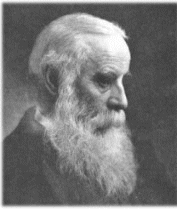
\includegraphics[scale=1]{../../graphics/wilson.jpg}
	\caption{John Cook Wilson}
	\label{fig:wilson}
\end{figure}

\section{Preliminaries}\label{sec:preliminaries} % (fold)

Cook Wilson's criticism of Stout account of the experience of primary qualities is focused on the case of extension and is organized around three sets of considerations of increasing generality:
    \begin{enumerate}
        \item Criticism of visual extension (the sensation that is, on Stout's view, involved in the visual perception of extension)
        \item Criticism of Stout's understanding of apparent size that motivates the postulation of visual extension
        \item A fundamental diagnosis of this in terms of a conflation of different senses of appearance talk.
    \end{enumerate}

% section preliminaries (end)

\section{Visual Extension}\label{sec:visual_extension} % (fold)

Cook Wilson makes four sets of remarks about the distinction between visual and real extension. The discussion builds on his discussion of representation. He emphasizes that the sense-representation differs in kind from what it represents. That the sense-representation is numerically distinct directly follows from Stout's representative realism, that sense-re\-pre\-sen\-ta\-tion mediates our knowledge of what it represents. Cook Wilson, however, is relying on the stronger claim that sense-representation and what it represents are not only numerically distinct, but distinct in kind. So far, Cook Wilson has offered two reasons for this further claim:
    \begin{itemize}
    	\item \emph{The Berkelean reasoning}: Only a sensation can resemble a sensation. So if visual and real extension were alike in kind, real extension would be a kind of sensation that can exist and change independently of being perceived, but this is a ``flagrantly absurdity''.
    	\item \emph{The phenomenological claim} that there is nothing in sensation which is spatial
    \end{itemize}
Neither are completely persuasive. The Berkelean reasoning is implausible, and it is unclear why a representative realist like Stout should accept the phenomenological claim. There's an \emph{ad hominem} reason for attributing to Stout the distinction in kind:
    \begin{itemize}
        \item Stout argues that sensible extension and real extension are distinct because there is no common measure. But if sensible extension and real extension are incommensurable, then they differ in kind.
    \end{itemize}
The problem with the \emph{ad hominem} reason is that it's not accepted by all representative realists, and so conclusions drawn on its basis would apply to Stout only. 

\begin{discussion}
	Indeed, Paul Snowdon observes that not all representative realists have accepted the distinction in kind. Consider the inner picture model where the parts of the inner picture are spatially structured and this structure corresponds to the spatial structure that obtains among external objects.
\end{discussion}


A. Given the Berkelean reasoning, visual extension represents something unlike itself, so real extension differs in kind from any figure that is presented to us in perception or visual imagination. What, then, is real extension? We cannot say. Stout is ``committed to something worse even than a `thing in itself', viz., to `an attribute in itself'''.

B. That real extension is of the same kind as visual extension presupposed by the science of geometry. Two considerations:
    \begin{enumerate}
    	\item Just as there could be no science of a thing in itself, there could be no science of extension of itself.
	    \item Constructive proofs in geometry presuppose that extension presented in perception and visual imagination is real extension. Such proofs proceed through a perceived or imagined figure. If visual extension differs in kind from real extension, then geometry would be applicable to visual extension alone.
    \end{enumerate}

C. The phenomenological difference between heat and color. The sensation of heat is felt in the affected part of the body. We experience color, in contrast, as clearly and distinctly located in the perceived external object. (This is the phenomenological difference that is reflected in ordinary language.) It follows that color cannot be representative of extension because we cannot perceive it except as extended---as inhering in an extended surface. Nor can we imagine otherwise. If we perceive color, we must perceive at the same time extension. % Cook Wilson supports this by observing that if we perceive adjacent homogenous colors we necessarily perceive their boundary.

    \begin{discussion}
        Tom Avery wondered how Cook Wilson's talk of ``locating'' a color in an extended surface should be understood. Is it meant to be a projectivist thesis of the kind that Boghossian and Velleman endorse? No, rather it is a phenomenological claim about how color figures in our experience---color is presented in experience as inhering in an extended surface. Cook Wilson's claim is thus more akin to Moore's intuition about the ``diaphaneity'' or ``transparency'' of color experience.
    
        Paul Snowdon asked why Cook Wilson is discussing color sensations. A representative realist need not take color sensations as mediating our perceptual knowledge of extension. Couldn't a representative realist assign geometrical structure directly to sensation? (Compare: Hume's impressions are spatially structured.) Perhaps, but it is a presupposition of the present discussion that the sensation that mediates our perceptual knowledge of extension differs in kind from extension. Cook Wilson's point is that, given this constraint, color sensation, if such there be, could not mediate our perceptual knowledge of extension.
    \end{discussion}

    \begin{discussion}
         Rory Madden suggested that perhaps Cook Wilson is exaggerating the difference between heat and color. After all the sensation of heat is bodily \emph{located}---extended through the affected part of the body. Paul Snowdon suggested that the following difference might remain---we may feel heat in the affected part of the body, but it lacks geometrical properties like straightness.
    \end{discussion}

D. Cook Wilson gives an independent reason for thinking that sensation lacks spatial content. Cook Wilson observes that if we perceive adjacent homogenous colors we necessarily perceive their boundary, and that this is a boundary in the surface in which the colors inhere. While color may be inseparable from extension, colors inhere in surfaces of external objects and not in the sensations that they elicit. It is thus either a confusion or a \emph{façon de parler} to speak of color \emph{sensation} as extended.
    \begin{quote}
        Accurately, then, the sensations, whether tactual or of colour, are \emph{not} extended, and the idea of extension is \emph{absolutely inapplicable} to them. (\emph{Statement and Inference}, 782)
    \end{quote}
Cook Wilson further claims that the subjectivity of visual extension \emph{wholly} depends on the the view that sensations are themselves extended, and so should be rejected.

% section visual_extension (end)

\section{Apparent and Real Size}\label{sec:apparent_and_real_size} % (fold)

Cook Wilson claims that Stout is confused about visual extension because of a confusion about  real and apparent size. Specifically, the subjectivity of visual extension gets motivated by the thought that the apparent size of a body contrasts with its real size. (Consider how two things of equal size visually appear when they are viewed at different distances from the perceiver. Despite being equal in size one looks or appears smaller than the other.) 

Cook Wilson's methodology here anticipates Austin:
    \begin{quote}
    	Just as ``representative and represented'' so ``real and apparent'' seem to me regular trap words, which cannot be safely used in any particular case without a most patient examination of their meaning and justification in the particular instance. (\emph{Statement and Inference}, 785)
    \end{quote}

Cook Wilson makes negative and positive remarks about real and apparent size.

\subsection{Negative Remarks}\label{sub:negative_remarks} % (fold)

A. Stout's theory seems committed to a form of subjective idealism. Sensible extension is not real extension since real extension is in space but sensible extension is not (by hypothesis, for the sake of \emph{reductio}). Things appear extended in space. However, by Stout's lights, the space in which things appear extended is not real. This seems to be committed to a form of subjective idealism.
    
B. Cook Wilson's strategy is to argue against Stout's claim that real and apparent size are incommensurable and then to draw out some implausible consequences from what remains of his view. 

First apparent size and real size must be commensurable. If apparent size is a \emph{size}, it has a measure. There must then be a common measure between real and apparent size. This seems implausible. The reasoning overgeneralizes. There would be no incommensurable measures, but there are. 

Cook Wilson however has an interesting subsidiary argument. How do we measure the real extension of a line? Well, we use a ruler. But by hypothesis it is merely the apparent extension of the ruler which is given in experience. You might think that we apply the apparent extension of the ruler to the apparent line. But this presupposes that real extensions are in the same ratio to one another as apparent extensions, and, hence, that real and apparent size are commensurable.

\begin{discussion}
    Paul Snowdon suggested that while apparent figures may lack determinate metrical properties, comparative judgements may yet be true of them---this apparent line appears twice the length of this other apparent line. Two observations. First, if the comparative structure is rich enough, it may determine a metric and so apparent figures couldn't have these comparative properties without the corresponding metrical properties. Second, even supposing that we can only make comparative judgments of size of apparent figures, Cook Wilson's argument would still run. In order for us to conclude that this real line is twice the length of another on the basis their appearance presupposes that real extensions are in the same ratio to apparent extensions.
\end{discussion}

But, further, how do we know that real and apparent extension are in proportion since real extensions are never the objects of perception? (Is this fair? Shouldn't the claim be that they are never the objects of \emph{direct} perception?) 

\end{document}
